\documentclass{config}
\usepackage{lipsum}
\usepackage{graphicx}
\usepackage{setspace}
\usepackage{amssymb}
\usepackage{listings}
\usepackage{appendix}
\usepackage{hyperref}




\newcommand{\lesss}{\rotatebox[origin=c]{90}{$\land$}}
\newcommand{\less}{\ \lesss\ }

\newcommand{\biggg}{\rotatebox[origin=c]{90}{$\lor$}}
\newcommand{\bg}{\ \biggg\ }

\lstdefinestyle{customc}{
  belowcaptionskip=1\baselineskip,
  breaklines=true,
  frame=L,
  xleftmargin=\parindent,
  language=C,
  showstringspaces=false,
  basicstyle=\footnotesize\ttfamily,
  keywordstyle=\bfseries\color{green!40!black},
  commentstyle=\itshape\color{purple!40!black},
  identifierstyle=\color{blue},
  stringstyle=\color{orange},
}

\lstdefinestyle{customasm}{
  belowcaptionskip=1\baselineskip,
  frame=L,
  xleftmargin=\parindent,
  language=[x86masm]Assembler,
  basicstyle=\footnotesize\ttfamily,
  commentstyle=\itshape\color{purple!40!black},
}

\lstset{escapechar=@,style=customc}


\title{Rapport ECL - Template} %Titre du fichier

\begin{document}
\lstset{language=[x86masm]Assembler} 
\begin{spacing}{1.2}
%----------- Informations du rapport ---------

\titre{Bureau d'Etude en Mécanique \\ Relais d'accessoires} %Titre du fichier .pdf

\enseignant{M. Hugues \textsc{Templier}}%Nom des élèves

\eleves{
        Aastha \textsc{Papneja} \\
        Jérôme \textsc{Plé} \\
		Alexandre \textsc{Ratieuville-Ogier}}%Nom des élèves

%----------- Initialisation -------------------
        
\fairemarges %Afficher les marges
\fairepagedegarde %Créer la page de garde
\tabledematieres %Créer la table de matières


%------------ Corps du rapport ----------------



%\begin{center}
%\includegraphics[scale=0.6]{carte_sabre_lite_image2.jpg}
%\captionof{figure}{Vu sur System Viewer de notre programme fonctionnant sur la carte SabreLite}
%\end{center}

\newpage
\section{Introduction}

Dans notre phase d'apprentissage des différentes notions en mécanique, nous avons comme objectif de concevoir un relais d'accessoires pour un réacteur d'avion.
Ce relais est un élément clef pour le réacteur. En effet, il permet notamment de démarrer le réacteur d'un avion.



\begin{center}
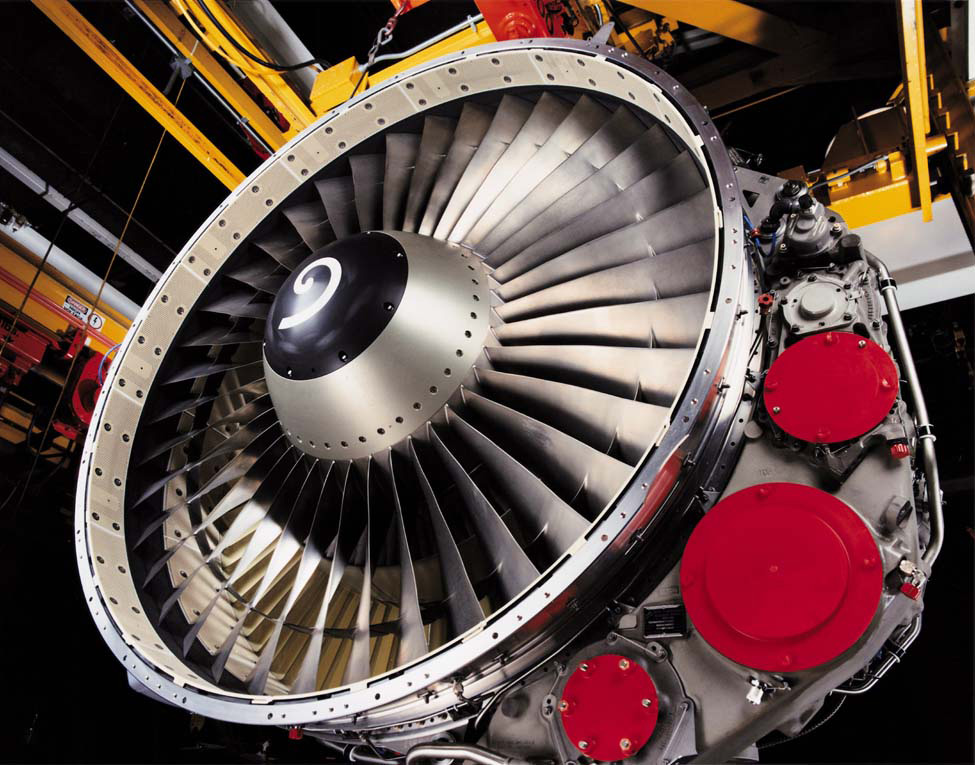
\includegraphics[scale=0.4]{CFM56-3C1-CFMi.jpg}
\captionof{figure}{Exemple d'un moteur à réaction en cours d'assemblage : le CFM56/General Electric F108}
\end{center}

De manière générale, ce relais d'accessoires se place dans la partie basse du moteur et aussi autour de la tuyère du réacteur.

\begin{center}
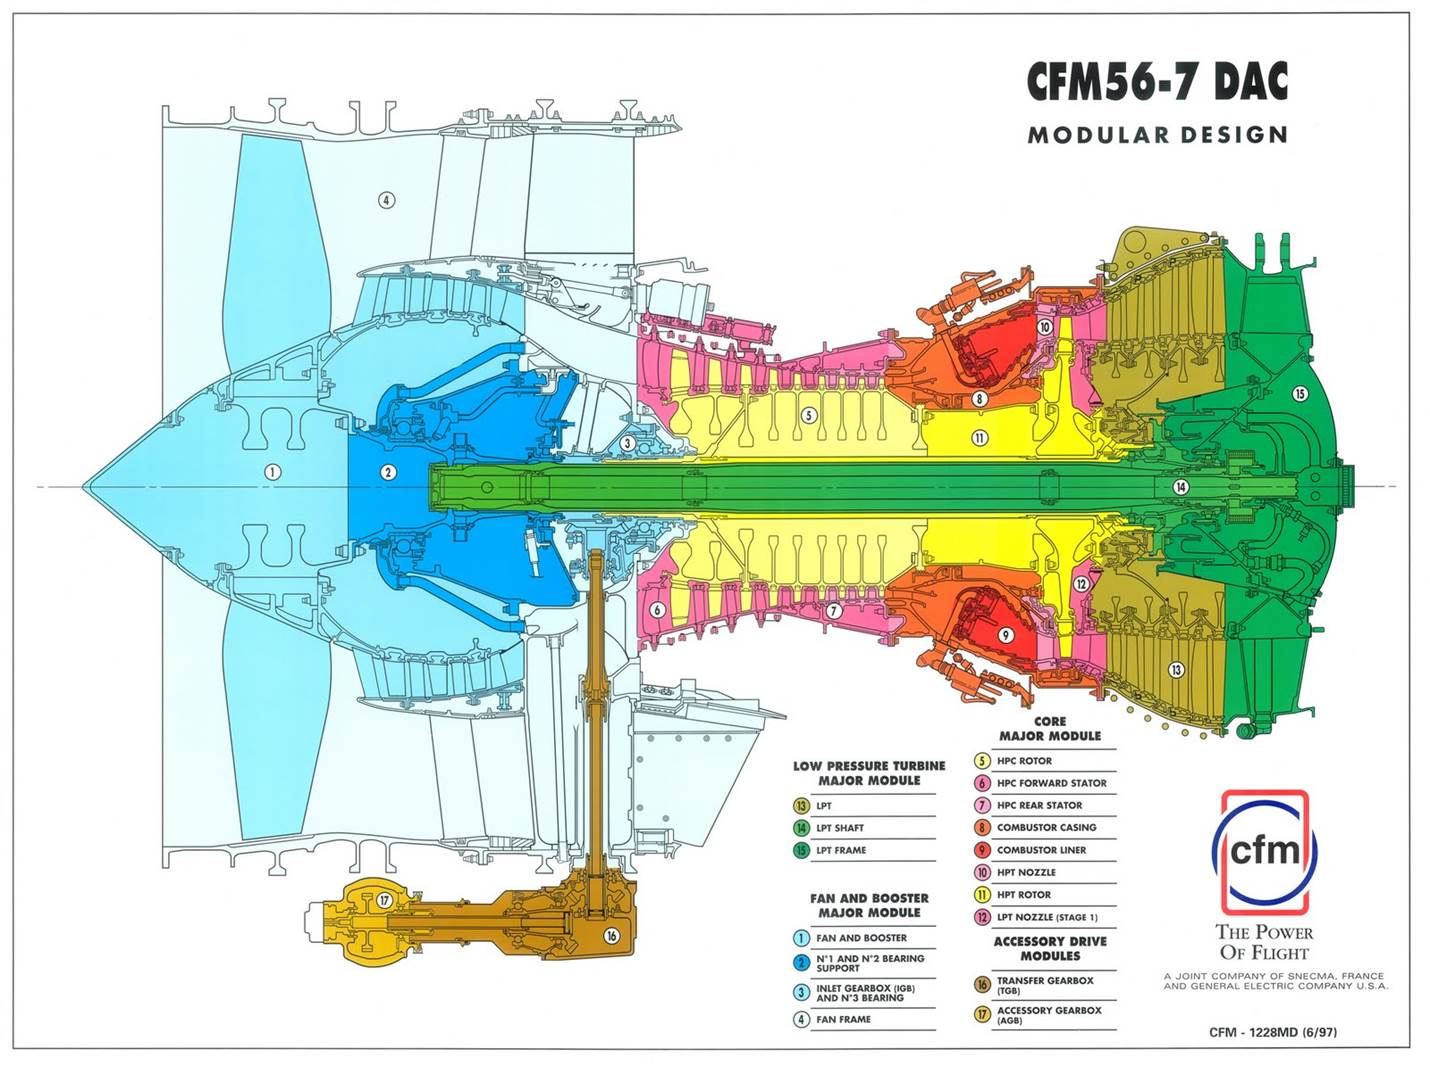
\includegraphics[scale=0.6]{CFM56-coupe.jpg}
\captionof{figure}{Vue de coupe du CFM56-7 DAC}
\end{center}

Comme nous pouvons le constater sur la vue en coupe du CFM56-7 DAC ci-dessus, le relais d'accessoires (qui est colorié en marron et possédant les numéros 16 et 17) est relié à l'arbre central du réacteur. Lors du démarrage du réacteur le démarreur fournit la rotation à l'arbre de la turbine, ce qui a pour effet de faire rentrer de l'air dans la tuyère. Une fois que le volume d'air dans la tuyère est suffisant, le carburant est injecté progressivement dans la zone de combustion. La rotation de la turbine se fait donc de plus en plus grâce à la combustion du carburant. Une fois que l'arbre central tourne suffisamment vite pour lui permettre de conserver son régime nominal en l'absence du démarreur, l'arbre du démarreur est débrayé.


\newpage
En regardant plus en profondeur un relais d'accessoires, nous remarquons la présence de nombreux composants et d'un jeu d'engrenage qui permet de faire la transmission de puissance entre les différents composants. La figure ci-dessous montre un relais d'accessoires de Rolls-Royce.
\begin{center}
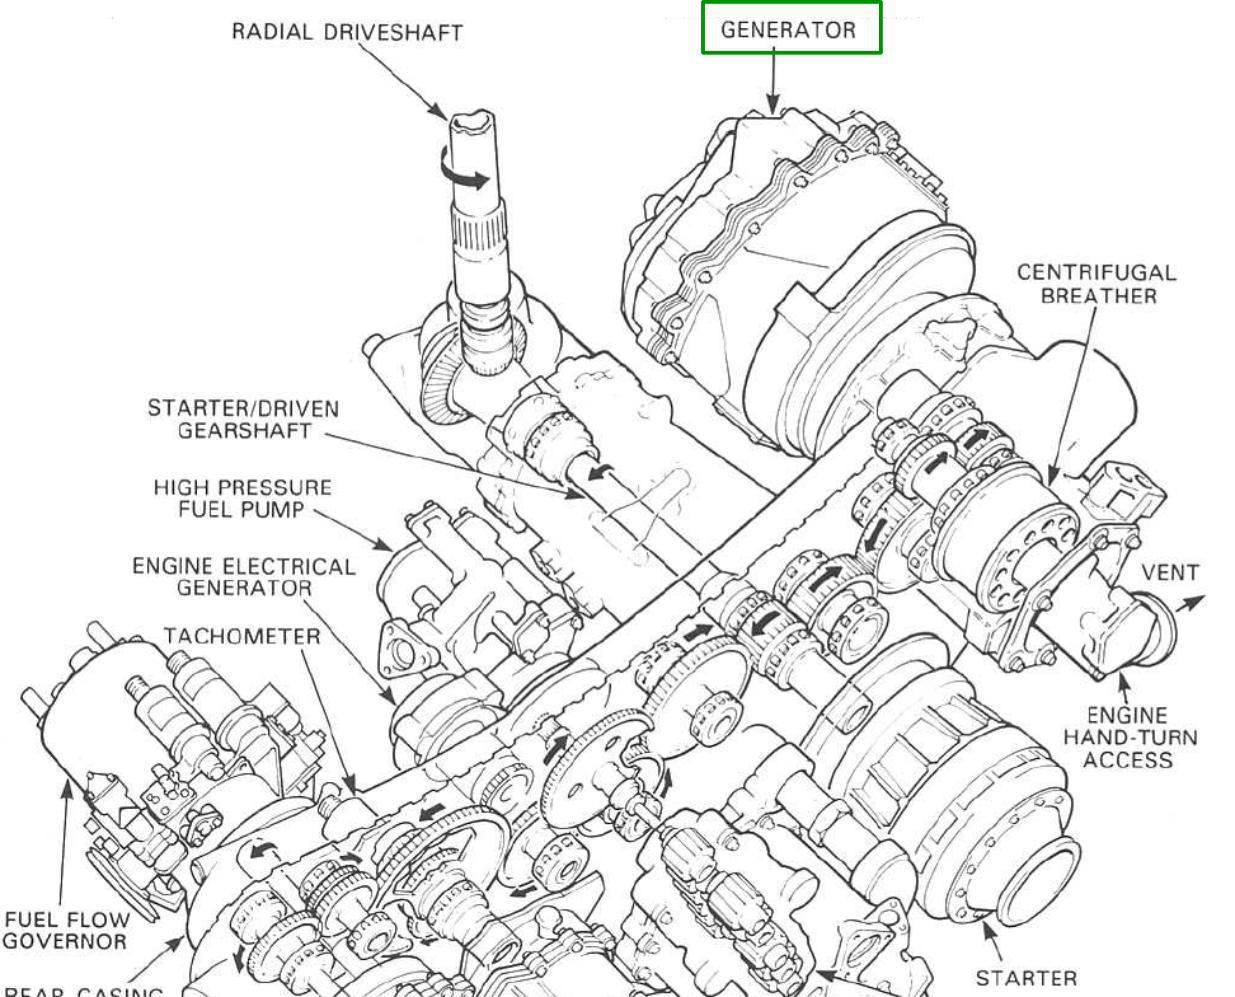
\includegraphics[scale=0.6]{relai_accessoires.jpg}
\captionof{figure}{Exemple d'un relais d'accessoires de Rolls-Royce}
\end{center}

Parmi les différents composants du relais d'accessoires, nous retrouvons une génératrice, un démarreur, des pompes hydrauliques et d'autres éléments indispensables pour le bon fonctionnement d'un avion. 

Il est important de signaler que les engrenages sont enfermés dans un carter et que ces engrenages sont imprégnés d'huile pour limiter les problèmes de contacts mécaniques. Une des pompe hydraulique est placé sur le relais d'accessoires pour permettre de maintenir un niveau d'huile suffisant dans le carter.

Dans le cadre de notre étude, nous allons concevoir un relais d'accessoires simplifié. En effet, nous devons réaliser ce relais en plaçant un démarreur, une génératrice et deux pompes hydrauliques.


\newpage
\section{Recherche de la meilleure configuration}

Pour notre étude, Cinq configurations matérielles sont possibles, chacune permettant de disposer les composants selon 2 architectures différentes. La première architecture vise à placer nos quatre composants du même côté alors que la deuxième architecture vise à placer deux composants de chaque côté.
La figure ci-dessous montre les deux architectures possibles. "P1" et "P2" représentent les pompes hydrauliques, "G" la génératrice et "D" le démarreur. 

\begin{center}
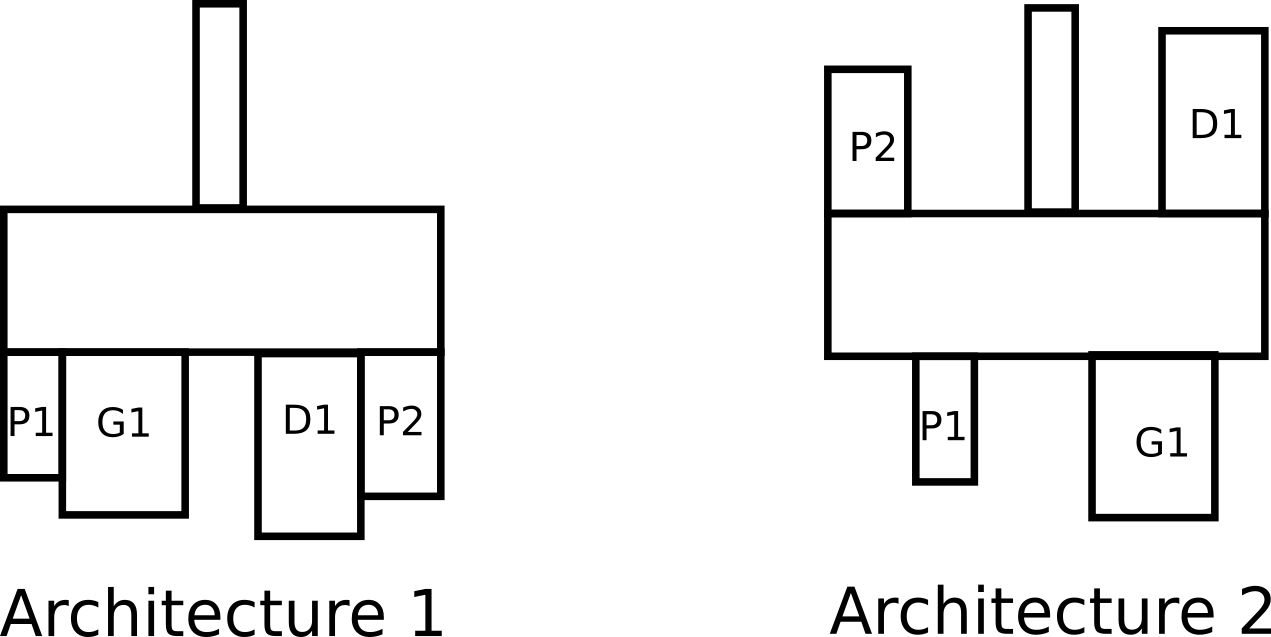
\includegraphics[scale=0.4]{architecture_BE.png}
\captionof{figure}{Les deux architectures possibles pour notre relais d'accessoires}
\end{center}

Au total, dix combinaisons sont possibles. Ci-dessous, un tableau récapitule les configurations possibles :

% Please add the following required packages to your document preamble:
% \usepackage{graphicx}
\begin{table}[h]
\centering
\resizebox{\textwidth}{!}{%
\begin{tabular}{|l|l|l|l|l|l|}
\hline
Configurations & Architecture & Démarreur & Générateur & Pompe 1 & Pompe 2 \\ \hline
A1/A2 & 1 ou 2 & D1 & G1 & P4 & P5 \\ \hline
B1/B2 & 1 ou 2 & D2 & G2 & P1 & P4 \\ \hline
C1/C2 & 1 ou 2 & D3 & G3 & P2 & P4 \\ \hline
D1/D2 & 1 ou 2 & D4 & G4 & P3 & P4 \\ \hline
E1/E2 & 1 ou 2 & D5 & G5 & P2 & P3 \\ \hline
\end{tabular}%
}
\end{table}

Afin de choisir la meilleure configuration, nous avons réalisé deux études. 

\begin{itemize}
 \item La première est une étude de l'encombrement de l'ensemble des composants selon la configuration.
 \item La deuxième est l'étude de la disposition des composants pour optimiser les rapports de réduction d'engrenage.
\end{itemize}

\newpage
\subsection{Étude de l'encombrement des différents composants}
Dans le but d'avoir un premier classement des différentes configurations matérielles, nous les avons ordonnées en fonction de l'encombrement qu'elles engendrent en considérant chaque accessoire du relais comme un cylindre de diamètre extérieur identique à celui de l'accessoire considéré. 

\begin{table}[h!]
\resizebox{\textwidth}{!}{%
\begin{tabular}{llllll}
\cline{1-5}
\multicolumn{1}{|l|}{Configuration} & \multicolumn{1}{l|}{Section cumulée cylindres}         & \multicolumn{1}{l|}{max diamètre (hauteur relais)}        & \multicolumn{1}{l|}{Profondeur}           & \multicolumn{1}{l|}{Puissance totale kW} &                                          \\ \cline{1-5}
\multicolumn{1}{|l|}{A1}            & \multicolumn{1}{l|}{69926}                                 & \multicolumn{1}{l|}{167}                                   & \multicolumn{1}{l|}{253}                  & \multicolumn{1}{l|}{123}                 &                                          \\ \cline{1-5}
\multicolumn{1}{|l|}{B1}            & \multicolumn{1}{l|}{76520}                                 & \multicolumn{1}{l|}{182}                                   & \multicolumn{1}{l|}{295}                  & \multicolumn{1}{l|}{173}                 &                                          \\ \cline{1-5}
\multicolumn{1}{|l|}{C1}            & \multicolumn{1}{l|}{115115}                                & \multicolumn{1}{l|}{244}                                   & \multicolumn{1}{l|}{378}                  & \multicolumn{1}{l|}{242}                 &                                          \\ \cline{1-5}
\multicolumn{1}{|l|}{D1}            & \multicolumn{1}{l|}{143184}                                & \multicolumn{1}{l|}{263}                                   & \multicolumn{1}{l|}{420}                  & \multicolumn{1}{l|}{271}                 &                                          \\ \cline{1-5}
\multicolumn{1}{|l|}{E1}            & \multicolumn{1}{l|}{168015}                                & \multicolumn{1}{l|}{287}                                   & \multicolumn{1}{l|}{450}                  & \multicolumn{1}{l|}{340}                 &                                          \\ \cline{1-5}
                                    &                                                            &                                                            &                                           &                                          &                                          \\ \hline
\multicolumn{1}{|l|}{Configuration} & \multicolumn{1}{l|}{Section cumulée, face 1} & \multicolumn{1}{l|}{Section cumulée, face 2} & \multicolumn{1}{l|}{Max(section cumulée)} & \multicolumn{1}{l|}{Profondeur}          & \multicolumn{1}{l|}{Puissance totale kW} \\ \hline
\multicolumn{1}{|l|}{A2}            & \multicolumn{1}{l|}{39107}                                 & \multicolumn{1}{l|}{38673}                                 & \multicolumn{1}{l|}{39107}                & \multicolumn{1}{l|}{460}                 & \multicolumn{1}{l|}{123}                 \\ \hline
\multicolumn{1}{|l|}{B2}            & \multicolumn{1}{l|}{43219}                                 & \multicolumn{1}{l|}{41155}                                 & \multicolumn{1}{l|}{43219}                & \multicolumn{1}{l|}{542}                 & \multicolumn{1}{l|}{173}                 \\ \hline
\multicolumn{1}{|l|}{C2}            & \multicolumn{1}{l|}{64905}                                 & \multicolumn{1}{l|}{58064}                                 & \multicolumn{1}{l|}{64905}                & \multicolumn{1}{l|}{708}                 & \multicolumn{1}{l|}{242}                 \\ \hline
\multicolumn{1}{|l|}{D2}            & \multicolumn{1}{l|}{75708}                                 & \multicolumn{1}{l|}{75330}                                 & \multicolumn{1}{l|}{75708}                & \multicolumn{1}{l|}{777}                 & \multicolumn{1}{l|}{271}                 \\ \hline
\multicolumn{1}{|l|}{E2}            & \multicolumn{1}{l|}{86075}                                 & \multicolumn{1}{l|}{89794}                                 & \multicolumn{1}{l|}{89794}                & \multicolumn{1}{l|}{835}                 & \multicolumn{1}{l|}{340}                 \\ \hline
\end{tabular}%
}
\caption{Classement ordonné par puissance consommée et encombrement des différentes configurations matérielles pour chaque architecture}
\end{table}

La configuration qui permet un encombrement minimal est ainsi la configuration A2, en disposant le démarreur du côté de l'arbre d'entrée E et la génératrice du côté opposé.

\newpage
\subsection{Étude des rapports de réduction}

Un premier classement ayant été réalisé concernant l'encombrement, nous nous intéressons maintenant à l'étude des rapports de réduction. 

En effet, un rapport de réduction compris entre 0,5 et 2 est demandé par l'énoncé pour chaque transmission par engrenage.\\
Cela aboutira à un deuxième classement, de la configuration la plus optimisée (le moins de changements de diamètres d'engrenages) à la moins optimisée.

Après automatisation informatique de cette classification, nous avons pu au total tester 480 combinaisons possibles ((1 (architecture 1) + 3 (architecture 2))$\times$ 4!$\times$ 5 (configurations) = 4$\times$24$\times$5 = 480). L'architecture 2 permet trois dispositions différentes car nous pouvons avoir le cas où les arbres de deux composants peuvent se connecter sur un arbre intermédiaire.

Pour effectuer un classement pertinent, nous avons décidé de classer les configurations en fonction la colonne \textit{écart-type}, du nombre d'engrenages ayant un rapport de réduction à l'extérieur de l'intervalle $[0,5,2]$ et du respect du sens de rotation du démarreur. En effet, en fonction de la configuration, le démarreur tourne dans le sens horaire ou dans le sens trigonométrique. 

La colonne \textit{écart-type} est un indicateur. Plus cet indicateur est important, plus cela signifie que la configuration calculée nécessite des changements de diamètre importants. 

Le tableau ci-dessous est un extrait de cette étude. Il analyse les différentes dispositions possibles pour la configuration A1.

% Please add the following required packages to your document preamble:
% \usepackage{graphicx}
\begin{table}[h]
\centering
\resizebox{\textwidth}{!}{%
\begin{tabular}{|l|l|l|l|l|l|}
\hline
Configuration & Entre 1 et 2 & Entre 2 et centre & Entre 3 et centre & Entre 4 et 3 & Écart-type \\ \hline
D1/G1/P4/P5 & 0,584 & 2,094 & 0,409 & 0,760 & 0,768513463 \\ \hline
D1/G1/P5/P4 & 0,584 & 2,094 & 0,311 & 1,316 & 0,80050416 \\ \hline
D1/P4/G1/P5 & 2,985 & 0,409 & 2,094 & 0,149 & 1,359131176 \\ \hline
D1/P5/G1/P4 & 3,929 & 0,311 & 2,094 & 0,195 & 1,760340963 \\ \hline
D1/P4/P5/G1 & 2,985 & 0,409 & 0,311 & 6,732 & 3,014414058 \\ \hline
D1/P5/P4/G1 & 3,929 & 0,311 & 0,409 & 5,115 & 2,45143273 \\ \hline
G1/D1/P4/P5 & 1,714 & 1,222 & 0,409 & 0,760 & 0,566371493 \\ \hline
G1/D1/P5/P4 & 1,714 & 1,222 & 0,311 & 1,316 & 0,592698574 \\ \hline
G1/P4/D1/P5 & 5,115 & 0,409 & 1,222 & 0,255 & 2,28308889 \\ \hline
G1/P5/D1/P4 & 6,732 & 0,311 & 1,222 & 0,335 & 3,083966172 \\ \hline
G1/P4/P5/D1 & 5,115 & 0,409 & 0,311 & 3,929 & 2,45143273 \\ \hline
G1/P5/P4/D1 & 6,732 & 0,311 & 0,409 & 2,985 & 3,014414058 \\ \hline
P4/G1/D1/P5 & 0,195 & 2,094 & 1,222 & 0,255 & 0,901206993 \\ \hline
P4/G1/P5/D1 & 0,195 & 2,094 & 0,311 & 3,929 & 1,760340963 \\ \hline
P4/D1/P5/G1 & 0,335 & 1,222 & 0,311 & 6,732 & 3,083966172 \\ \hline
P4/D1/G1/P5 & 0,335 & 1,222 & 2,094 & 0,255 & 0,864661744 \\ \hline
P4/P5/D1/G1 & 1,316 & 0,311 & 1,222 & 1,714 & 0,592698574 \\ \hline
P4/P5/G1/D1 & 1,316 & 0,311 & 2,094 & 0,584 & 0,80050416 \\ \hline
P5/D1/G1/P4 & 0,255 & 1,222 & 2,094 & 0,195 & 0,901206993 \\ \hline
P5/P4/G1/D1 & 0,760 & 0,409 & 2,094 & 0,584 & 0,768513463 \\ \hline
P5/P4/D1/G1 & 0,760 & 0,409 & 1,222 & 1,714 & 0,566371493 \\ \hline
P5/G1/P4/D1 & 0,149 & 2,094 & 0,409 & 2,985 & 1,359131176 \\ \hline
P5/D1/P4/G1 & 0,255 & 1,222 & 0,409 & 5,115 & 2,28308889 \\ \hline
P5/G1/D1/P4 & 0,149 & 2,094 & 1,222 & 0,335 & 0,895250311 \\ \hline
\end{tabular}%
}
\end{table}
\newpage

Le graphique ci-dessous est représentatif de l'optimisation dans la disposition des accessoires. La configuration la plus intéressante minimisant les changements de diamètre des engrenages est donc G1/D1/P4/P5 pour l'architecture A1 (toutes les pièces du même côté).

\begin{center}
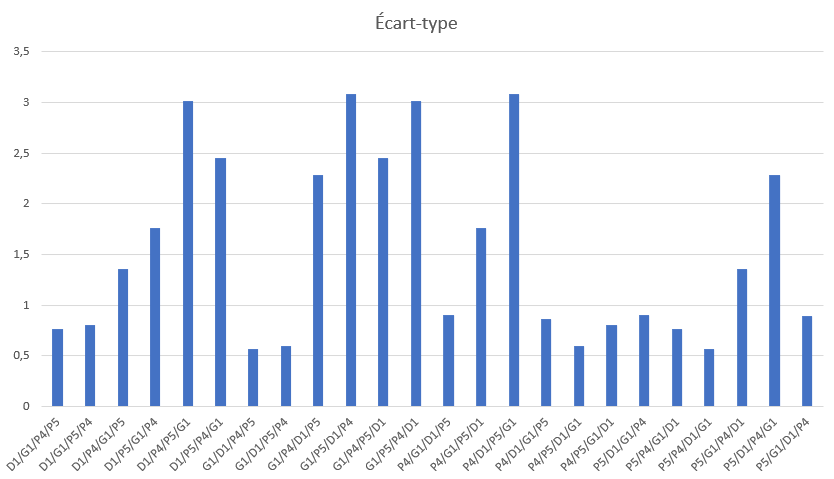
\includegraphics[scale=0.8]{graphique_ecart_type.PNG}
\captionof{figure}{Courbe récapitulant l'écart type pour la configuration A1}
\end{center}

Pour chaque configuration, nous avons testé l'ensemble des combinaisons possibles et affiché l'écart-type pour les quatre architectures possibles pour la configuration. La figure ci-dessous montre l'écart-type des différentes combinaisons possibles avec la configuration A.

\begin{center}
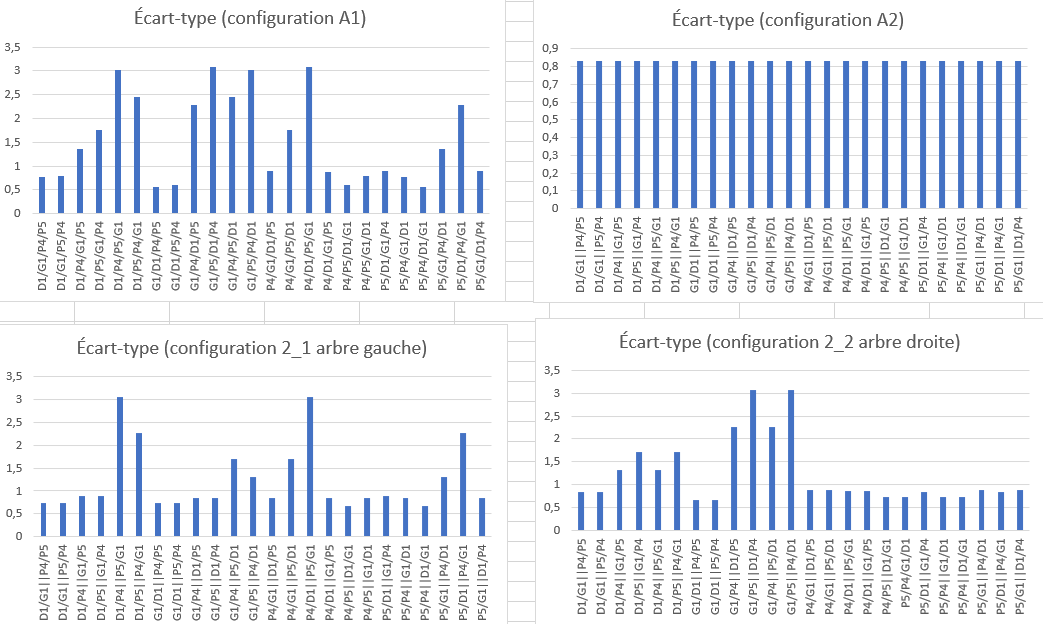
\includegraphics[scale=0.75]{graphique_ecart_type_configurationA.PNG}
\captionof{figure}{Courbes de l'écart-type des différentes combinaisons possibles avec la configuration A}
\end{center}

De cette étude, nous avons retenu les configurations suivantes : G1/D1/P4/P5 et G1/D1/P5/P4.

\newpage
\begin{center}
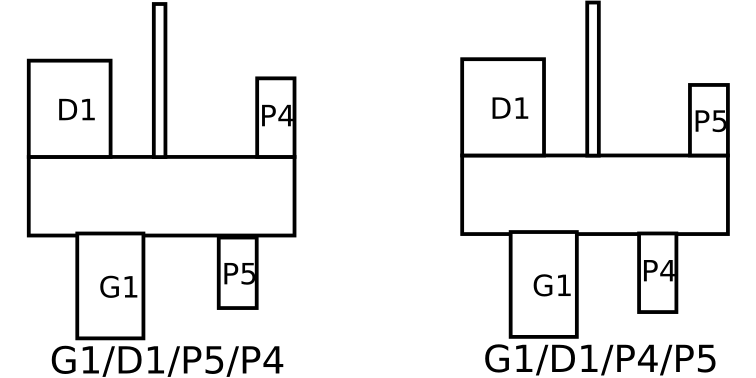
\includegraphics[width=\textwidth]{conf_retenu.png}
\captionof{figure}{Les configurations retenues par notre équipe}
\end{center}

Le choix entre ces deux configurations sera fait en fonction de l'espace disponible.

Notons que dans cette étude le \textbf{démarreur} est supposé tourner à \textbf{11000 tr/min}.

\newpage
\section{Étude dans le cas d'un fonctionnement nominal}

Dans cette partie, nous nous sommes intéressés à dimensionner notre relais d'accessoires lorsque ce dernier fonctionne à régime nominal. 

Lors de notre étude pour déterminer la meilleure configuration, nous avons pu constater que la configuration A2 nécessite un arbre intermédiaire pour adapter les vitesses de rotations avec des rapports de réductions compris entre  0,5 et 2.

BESOIN DU SCHEMA DE JEROME AVEC UN SEUL INTERMEDIAIRE

Vous trouverez ci-dessous le tableau récapitulatif des contraintes pour chaque composant de notre relais d'accessoires.

% Please add the following required packages to your document preamble:
% \usepackage{graphicx}
\begin{table}[h]
\centering
\resizebox{\textwidth}{!}{%
\begin{tabular}{|l|l|l|l|l|}
\hline
COMPOSANT & Puissance (W) & Vitesse de rotation (rpm) & Vitesse de rotation (rads-1) & Couple (Nm) \\ \hline
Démarreur & 8,20E+04 & 11000 & 1 151,92 & 71,19 \\ \hline
Génératrice & 2,00E+04 & 18850 & 1 973,97 & 10,13 \\ \hline
Pompe 4 & 1,89E+04 & 3685 & 385,89 & 49,00 \\ \hline
Pompe 5 & 4,46E+03 & 2800 & 293,22 & 15,21 \\ \hline
Intermédiaire & 0,00E+00 & 4500 & 471,24 & 0,00 \\ \hline
TOTAL & 1,25E+05 &  &  &  \\ \hline
\end{tabular}%
}
\end{table}

\subsection{Dimensionnement préliminaire des arbres}
Afin de dimensionner correctement les arbres de notre système, il est nécessaire de calculer le couple subis par chacun de ces arbres et de déterminer leur diamètre minimal. Vous trouverez ci-dessous le tableau récapitulatif des efforts subis par chaque arbre.

% Please add the following required packages to your document preamble:
% \usepackage{graphicx}
\begin{table}[h]
\centering
\resizebox{\textwidth}{!}{%
\begin{tabular}{|l|l|l|l|l|}
\hline
ARBRE & Puissance (W) & Vitesse de rotation (rpm) & Vitesse de rotation (rads-1) & Couple (Nm) \\ \hline
Arbre Entrée & 1,25E+05 & 9000 & 942,48 & 133,02 \\ \hline
Arbre Démarreur & 1,02E+05 & 11000 & 1 151,92 & 88,55 \\ \hline
Arbre Génératrice & 2,00E+04 & 18850 & 1 973,97 & 10,13 \\ \hline
Arbre Intermédiaire & 2,34E+04 & 4500 & 471,24 & 49,59 \\ \hline
Arbre Pompe 4 & 1,89E+04 & 3685 & 385,89 & 49,00 \\ \hline
Arbre Pompe 5 & 4,46E+03 & 2800 & 293,22 & 15,21 \\ \hline
\end{tabular}%
}
\end{table}

En connaissant les couples pour chaque arbre, nous avons pu calculer le diamètre minimal pour chacun d'entre eux.

\begin{table}[h]
\centering
\begin{tabular}{|l|l|l|}
\hline
DIAMÈTRE & Diamètre mini (mm) & Diamètre min (Pire des cas) \\ \hline
Arbre Entrée & 22,73 & 22,81 \\ \hline
Arbre Démarreur & 19,85 & 19,91 \\ \hline
Arbre Génératrice & 9,64 & 9,67 \\ \hline
Arbre Intermédiaire & 16,36 & 16,41 \\ \hline
Arbre Pompe 4 & 16,29 & 16,35 \\ \hline
Arbre Pompe 5 & 11,03 & 11,07 \\ \hline
\end{tabular}
\end{table}

Lors de cette étude, nous avons étudié le diamètre minimal lorsque les vitesses de rotations sont parfaitement respectées et aussi lorsque nous avons une erreur de 1\% pour chaque vitesse de rotation. Cette erreur de 1 \% correspond à la valeur maximale autorisée par notre cahier des charges fonctionnel.

En connaissant les diamètres minimales, nous avons pu obtenir un ordre de grandeur pour les diamètres de nos arbres. Cependant, nous avons effectué le dimensionnement préliminaire des autres composants avant de choisir définitivement les diamètres.

\newpage
\subsection{Dimensionnement des clavettes/cannelures}
Afin de transmettre les efforts mécaniques aux engrenages, il est nécessaire d'utiliser des clavettes ou des cannelures. 

Le choix entre ces différents montages dépend des efforts à transmettre et du diamètre de l'arbre.

\subsubsection{Étude des clavettes}
A titre de première piste explorée, nous avons étudié les clavettes. Les clavettes sont couramment utilisés grâce à leur facilité d'intégration sur un arbre.
\begin{center}
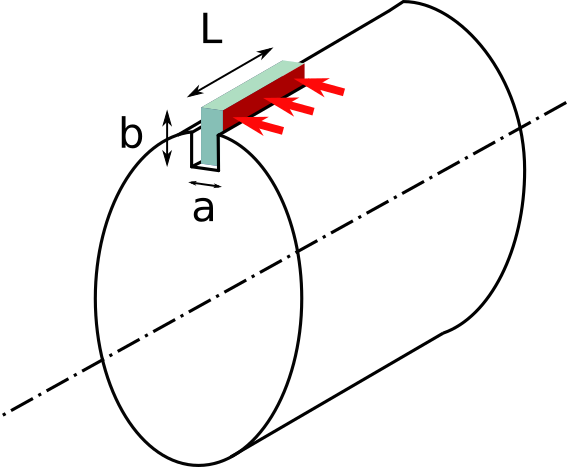
\includegraphics[width=0.5\textwidth]{Determination_clavette_sur_arbre.png}
\captionof{figure}{Représentation de la surface de matage d'une clavette}
\end{center}

La clavette est matée si 
\[P_n = \frac{F_n}{S_n}  \geq 50 MPa \]
Nous avons une pression de matage de 50 MPa car c'est la valeur que nous avions utilisé pour l'étude du concasseur durant nos séances de Bureau d'Etude Mécanique.
Nous choisissons donc $S_n$ surface de contact où les forces s'appliquent de manière à vérifier ce critère.
\[S_n = \frac{b}{2}L  \]
D'où  \[L>= \frac{b}{2}\frac{P_n}{F_n}\]

A titre d'exemple, prenons le cas de l'arbre d'entrée. Nous rappelons qu'il est nécessaire que le diamètre minimal de l'arbre est de 22,81 mm dans le pire des cas. De même, le couple à transmettre est de 133,02 Nm. 
Pour ajouter une clavette sur notre arbre, il est nécessaire de diminuer localement le diamètre de l'arbre. Par conséquent, nous proposons de prendre un diamètre de 28 mm pour éviter une fragilisation trop importante de l'arbre. 

Par application numérique, nous trouvons que $F_n = 4,4 kN$ et qu'avec b = 8 mm, $L => 45 mm$

En réalisant d'autres calculs pour les autres arbres, nous nous sommes rendus comptes que nous avons plusieurs longueurs de clavettes supérieures à 30 mm. De telles longueurs nous obligent ne placer des épaulements à proximité des engrenages ce qui ne rend pas l'assemblage facilement faisable et compromet en partie la compacité du relais d'accessoires.

Au vu des résultats plus non concluants avec les clavettes, nous avons décidé de nous tourner vers les cannelures.

\subsubsection{Étude des cannelures}
Après étudié les clavettes, nous avons étudié l'autre façon de transmettre les efforts mécaniques d'un arbre vers un engrenage : les cannelures.


Il existe deux types de cannelures : les cannelures à flancs parallèles et les cannelures à flancs en développante.
Dans la suite, nous avons présenter nos calculs pour les deux types de cannelures.

\paragraph{Étude des cannelures à flancs parallèles}

Lorsqu'il n'est pas possible d'utiliser des clavettes pour des raisons de longueur trop importantes, il est recommandé d'étudier les cannelures à flancs parallèles.

\begin{center}
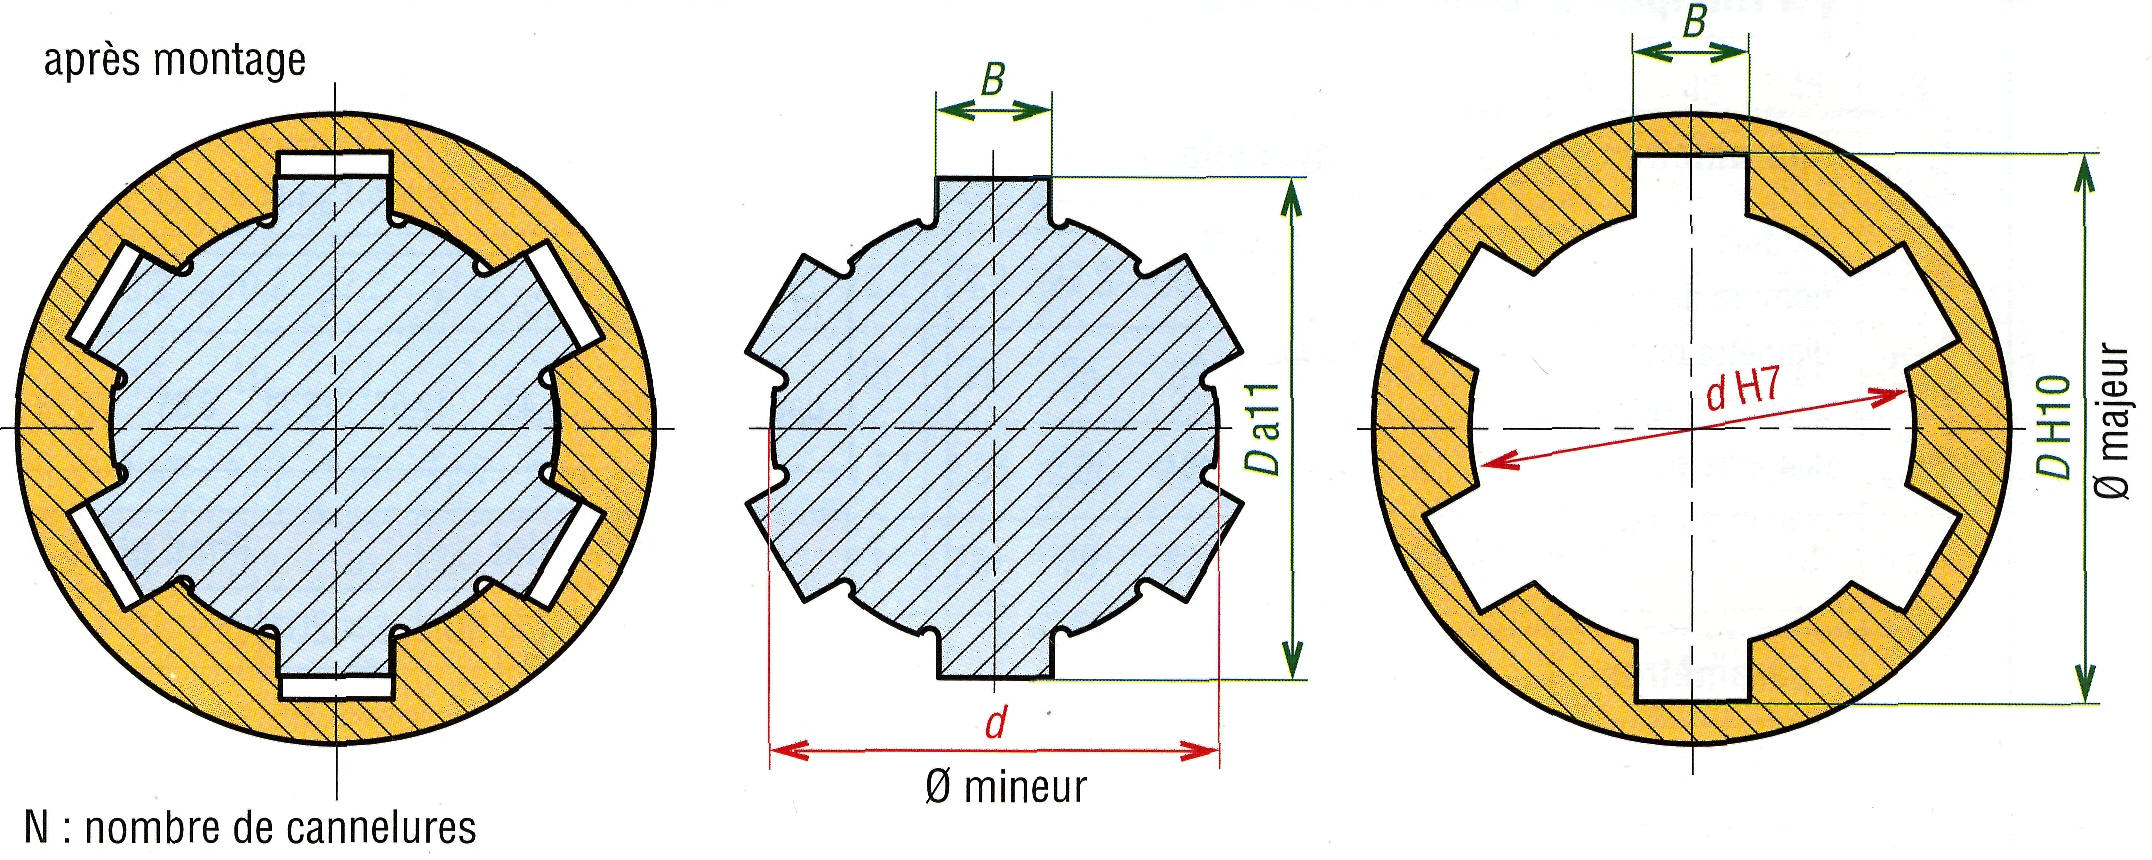
\includegraphics[width=0.8\textwidth]{cannelure_parallele.jpg}
\captionof{figure}{Représentation d'une cannelure à flancs parallèles}
\end{center}

Afin de dimensionner ces cannelures, il est nécessaire d'effectuer l'hypothèse que la répartition de la pression est uniforme sur les flancs surface portante à 75 \% de la surface (A).

Nous posons les notations suivantes :
\begin{itemize}
\item n : nombre de cannelures
\item h : hauteur d'une cannelure
\item C : couple à transmettre
\item p : pression de contact
\item L : longueur des cannelures
\item Dm : diamètre moyen : (D+d)/2
\end{itemize}

Nous pouvons alors poser les équations suivantes :

\begin{itemize}
    \item Surface de contact : A = (3/4).n.h
    \item Couple transmissible : C = (p.A.L.Dm) / 2
    \item Condition de non matage : p= 2.C / A.L.Dm =<  Padm
\end{itemize}

En nous appuyant sur ces formules, nous pouvons détemriner que la longueur

\begin{center}
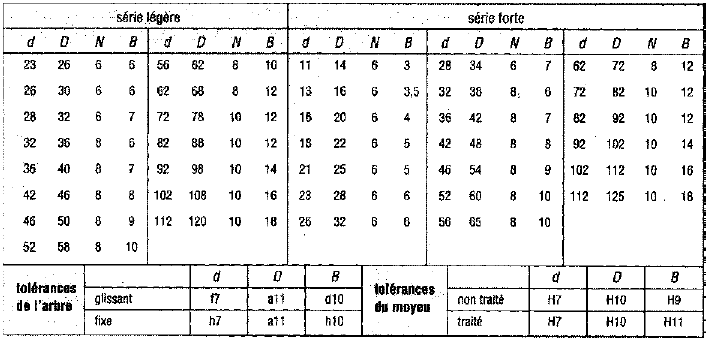
\includegraphics[width=0.8\textwidth]{tab_cannelures.PNG}
\captionof{figure}{Représentation d'une cannelure à flancs parallèles}
\end{center}
    



\subsection{Dimensionnement des engrenages}

\subsection{Dimensionnement des roulements et des entroises}

\subsection{Modélisation sur CATIA}


\section{Étude dans le cas du démarrage de notre relais d'accessoires}

\subsection{Dimensionnement des arbres}

\subsection{Dimensionnement des cannelures}

\subsection{Dimensionnement des engrenages}

\subsection{Dimensionnement des roulements et des entroises}

\subsection{Modélisation sur CATIA}

\end{spacing}
\end{document}

